\documentclass[11pt,aspectratio=169]{beamer}
\usetheme{Madrid}

% ---------- Encoding / micro-typography ----------
\usepackage[tracking=alltext,letterspace=-15]{microtype}
\SetExtraKerning
  [ name = english-default, context = english, unit = space ]
  { encoding = {OT1,T1,LY1} }
  { f = {,1000}, r = {,1000} }

% ---------- Math & symbols ----------
\usepackage{mathtools}
\usepackage{amssymb,amsfonts}
\usepackage{bm}
\usepackage{bbm}
\usepackage{cancel}
\usepackage{pifont}

% ---------- Graphics / colors / tables ----------
\usepackage{graphicx}
\usepackage[table]{xcolor}
\usepackage{colortbl}
\usepackage{booktabs}
\usepackage{multirow}
\usepackage{threeparttable}

% ---------- Drawing / boxes / highlighting ----------
\usepackage{tikz}
\usepackage[most]{tcolorbox}
\usepackage[normalem]{ulem}
\usepackage{soul}

% ---------- Animation ----------
\usepackage{animate}

% ---------- Bibliography ----------
\usepackage{natbib}
\usepackage{hanging}
\pdfstringdefDisableCommands{\def\translate#1{#1}}



% ==================================================
%                 COLOR PALETTE
% ==================================================

% Core pink theme
\definecolor{darkpink}{RGB}{139,0,75}        % deep elegant pink
\definecolor{softpink}{RGB}{214,112,147}     % lighter accent
\definecolor{lightsoftpink}{RGB}{250,225,235}

% Accent colors (kept from your original palette)
\definecolor{highlightcolor}{HTML}{C70039}
\definecolor{burgundy}{rgb}{0.5,0.0,0.13}
\definecolor{arsenic}{rgb}{0.23,0.27,0.29}
\definecolor{darkorange}{rgb}{1.0,0.55,0.0}
\definecolor{mblue}{rgb}{0.0,0.4470,0.7410}
\definecolor{forest_Periwinkle}{rgb}{0.3333,0.4588,0.1843}
\definecolor{bubbles}{rgb}{0.91,1.0,1.0}
\definecolor{boldblue}{rgb}{0.2,0.2,0.6}
\definecolor{boldcolor}{rgb}{0.5,0.0,1.0}
\definecolor{minorbold}{rgb}{0.0,0.5,1.0}
\definecolor{boldPeriwinkle}{rgb}{0.0,0.5,0.0}
\definecolor{boldred}{rgb}{0.5,0.0,0.0}

% Main accent color (used in transitions & bullets)
\definecolor{maincolor}{RGB}{139,0,75}

% ==================================================
%              BEAMER LOOK-AND-FEEL
% ==================================================

% Frame titles
\setbeamercolor{frametitle}{fg=white,bg=darkpink}
\setbeamertemplate{frametitle}{%
  \nointerlineskip%
  \begin{beamercolorbox}[wd=\paperwidth,ht=3ex,dp=1.5ex,leftskip=0.7cm]{frametitle}
    \insertframetitle
  \end{beamercolorbox}%
}

% Structure color (bullets, numbering, etc.)
\setbeamercolor{structure}{fg=darkpink}

% Progress bar
\setbeamercolor{progress bar}{fg=darkpink,bg=darkpink!20}

% Title page text
\setbeamercolor{title}{fg=darkpink}
\setbeamercolor{subtitle}{fg=darkpink}
\setbeamercolor{title separator}{fg=darkpink}

% Background
\setbeamercolor{background canvas}{bg=white}

% Blocks
\setbeamercolor{block title}{bg=darkpink,fg=white}
\setbeamercolor{block body}{bg=lightsoftpink,fg=black}

% Remove footline
\setbeamertemplate{footline}{}
\addtobeamertemplate{title page}{\vspace*{-0.5\baselineskip}}{}

% ==================================================
%               THEOREMS
% ==================================================

\newtheorem{prop}{Proposition}

\usepackage{etoolbox}
\AtBeginEnvironment{prop}{%
  \setbeamercolor{block title}{bg=darkpink,fg=white}%
  \setbeamercolor{block body}{bg=lightsoftpink,fg=black}%
}

% ==================================================
%               CONVENIENCE
% ==================================================

\newcolumntype{B}{>{\columncolor{bubbles}}c}
\setbeamertemplate{itemize items}[circle]
\setbeamertemplate{itemize subitem}{\tiny\raise1.5pt\hbox{\donotcoloroutermaths$\color{maincolor}\blacktriangleright$}}
\setbeamertemplate{itemize subsubitem}{\scriptsize\raise1.5pt\hbox{\donotcoloroutermaths$\color{maincolor}\bullet$}}

\newcommand{\xmark}{\ding{55}}
\newcommand{\cmark}{\ding{51}}

% ---------- Tiny TikZ +/- ----------
\newcommand{\Plus}{\mathord{\begin{tikzpicture}[baseline=0ex,line width=1,scale=0.13]
  \draw (1,0) -- (1,2); \draw (0,1) -- (2,1);\end{tikzpicture}}}
\newcommand{\Minus}{\mathord{\begin{tikzpicture}[baseline=0ex,line width=1,scale=0.13]
  \draw (0,1) -- (2,1);\end{tikzpicture}}}

% ---------- Coloured table helpers ----------
\newcommand{\noch}{\cellcolor{arsenic}{\color{white}{0}}}
\newcommand{\gup}{\cellcolor{forest_Periwinkle}{\color{white}{+}}}
\newcommand{\gdown}{\cellcolor{burgundy}{\color{white}{-}}}
\newcommand{\idk}{\cellcolor{mblue}{\color{white}{?}}}

% ---------- Emphasis helpers ----------
\newcommand{\cemph}[1]{\color{boldcolor}#1\color{black}}
\newcommand{\chemph}[1]{\color{highlightcolor}#1\color{black}}

% Margins
\setbeamersize{text margin left=2em, text margin right=2em}
\addtolength{\leftmargini}{2em} 

% ---------- Proof symbol ----------
\renewcommand{\qedsymbol}{\textcolor{black}{\ensuremath{\square}}}

% ---------- Shortcuts ----------
\newcommand{\E}{\mathbb{E}}
\newcommand{\R}{\mathbb{R}}
\newcommand{\B}{\mathcal{B}}
\newcommand{\Cov}{\operatorname{Cov}}
\DeclareMathOperator*{\argmax}{arg\,max}
\DeclareMathOperator*{\argmin}{arg\,min}
\newcommand{\pbf}{$^{\mathbf +}$}
\newcommand{\bit}[1]{\begin{itemize}\setlength\itemsep{#1}}
\newcommand{\eit}{\end{itemize}}

% Transition title helper
\newcommand{\transitiontitle}[1]{%
  \frame[noframenumbering,c]{\frametitle{} \centering \LARGE \textbf{\color{maincolor} #1}}%
}


%%%%%%%%%%% ------ TITLE PAGE --------- %%%%%%%%%%%%%%%%%%%
\title{The Effect of Female Leadership on the Wage-Productivity Gap: Evidence from Colombian Manufacturing Firm Data \\ 
{\small Applied Microeconomic Theory ECON 6301 Paper}}
\author{Ingri Katherine Quevedo Rocha}
\institute{\small \url{ingriq@gwu.edu} \\ George Washington University \\ M.S. Applied Economics (Spring 2026)}
\date{\today}


%%%%%%%%%%%%%%%%%%%%%%%%%%% BEGIN %%%%%%%%%%%%%%%%%%%%%%%
\begin{document}

\begin{frame}
  \titlepage
\end{frame}


%%%%%%----------------------%%%%%%
\begin{frame}{Microeconomic Theory: How Wages Are Set in an Ideal World}

\begin{itemize}
  \item Many firms compete to hire workers
  \item Workers can easily switch jobs
  \item Wages reflect how much workers contribute to production
\end{itemize}

\begin{figure}
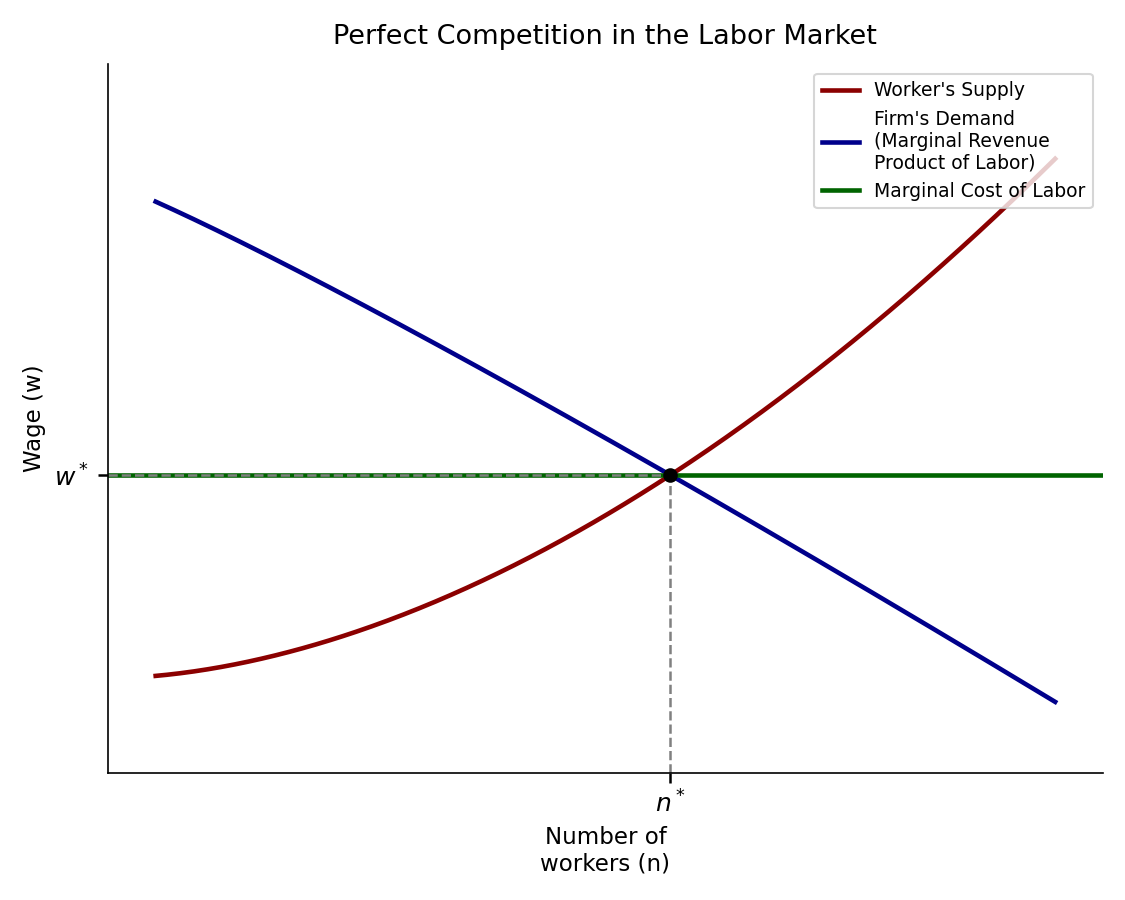
\includegraphics[width=0.6\textwidth]{example_perfect_competition.png}
\end{figure}

\end{frame}

%%%%%%----------------------%%%%%%
\begin{frame}{Microeconomic Theory: When Firms Have Power Over Workers}

\begin{itemize}
  \item Fewer job options for workers
  \item Switching jobs is costly or risky
  \item Firms can influence wages
\end{itemize}

\begin{figure}
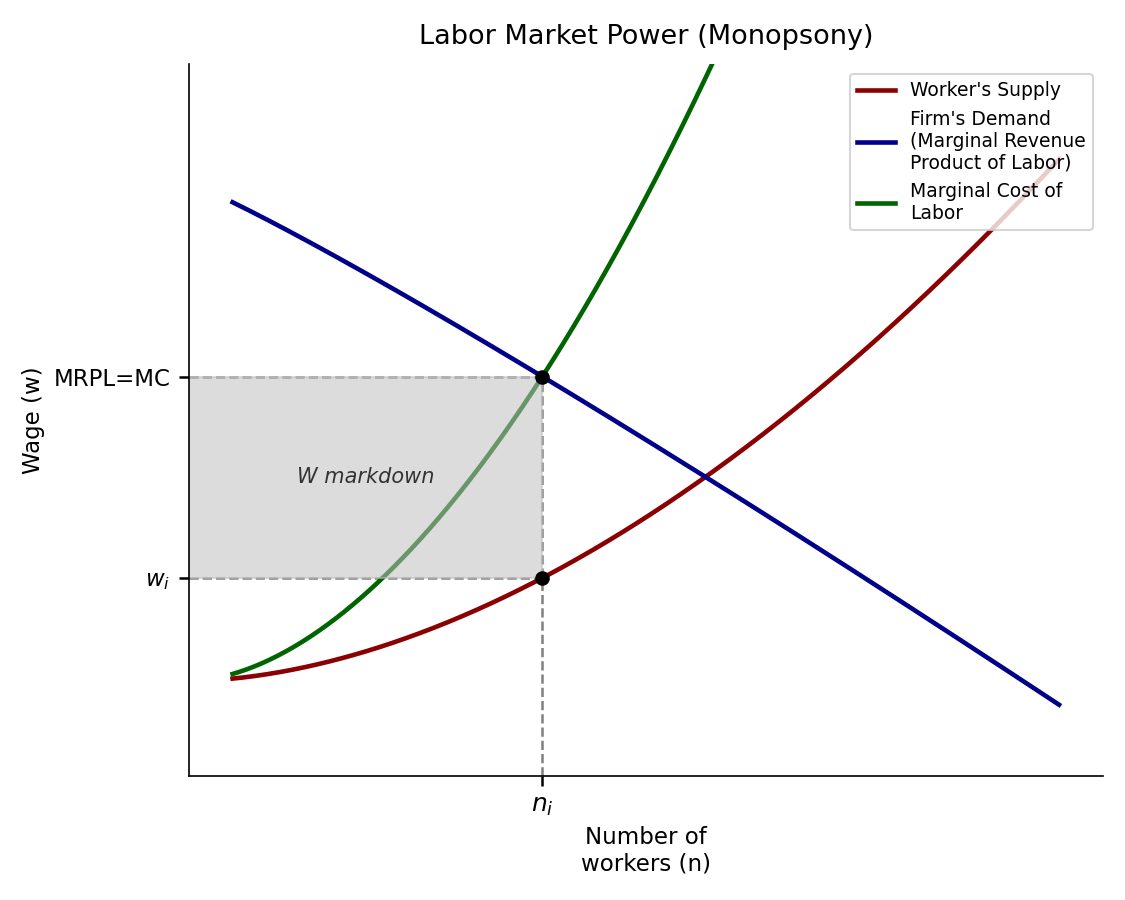
\includegraphics[width=0.6\textwidth]{example_labor_marker_power.png}
\end{figure}

\end{frame}


%%%%%%----------------------%%%%%%
\begin{frame}[t]{Research Question: Do women-led firms have lower labor markdowns?}
\vspace{-0.5cm}
\begin{equation}
  Markdown_{it} = \beta_{0} + \beta_{1} ShareFemaleOwners_{it} + \Phi Controls_{it} + \epsilon_{it} 
\end{equation}
\vspace{-0.5cm}
  \begin{block}{Expected $\beta{1}<0$}
    \begin{itemize}
      \item Management choices shape wage-setting and competition \cite{bertrand_is_1998}
      \item Firms differ systematically in management practices \cite{bloom_measuring_2007}
      \item Labor market power affects women more strongly (\cite{hirsch_differences_2010}, \cite{sharma_monopsony_2023})
      \item Female leaders reduce gender-specific wage distortions (\cite{flabbi_female_2017}, \cite{flabbi_female_2019})
      \item Firms with female leadership are less likely to downsize and pursue value-destroying consolidation \cite{matsa_female_2013}, \cite{levi_director_2014}, \cite{matsa_workforce_2014}
    \end{itemize}
  \end{block}
\end{frame}

%%%%%%----------------------%%%%%%
\begin{frame}[t]{Brief Literature Review}
\textbf{1. Labor market power and markdowns}
\begin{itemize}
  \item Labor market power is widespread: it can arise from employer concentration, job amenities, or information/search frictions  (\cite{manning_elusive_2021}; \cite{card_who_2022}; \cite{azar_minimum_2019}; \cite{manning_monopsony_2013}; \cite{lentz_labor_2010}; \cite{moscarini_unemployment_2010}), or higher concentration to lower wages (\cite{azar_labor_2017}; \cite{azar_minimum_2019}; \cite{benmelech_strong_2018}; \cite{rinz_labor_2022}).
\end{itemize}

\textbf{2. Latin America / Colombia evidence}
\begin{itemize}
  \item In Latin America and the Caribbean workers receive about half of what they contribute on average. In contrast, workers in the U.S. and advanced economies receive 65 percent and 81 percent, respectively.
  \item Colombia: estimated firm-level labor supply elasticity $\approx$ 2.5, implying workers produce about 40\% more than they earn (\cite{amodio_measuring_2024}).
\end{itemize}
\end{frame}

\begin{frame}[t]{Brief Literature Review}
\textbf{3. Gender, leadership, and firm behavior}
\begin{itemize}
  \item Female leadership correlates with firm performance in Latin America \cite{flabbi_female_2017} and with improved productivity and employment stability in U.S. firms (\cite{tunyi_doing_2023}, \cite{matsa_workforce_2014}).
  \item Gender differences in labor market power matter: in Chile, differences in labor supply elasticities imply men would earn about 22\% more than women \cite{sanchez_gender_2022}
  \item Female executives may reduce gender-specific wage distortions by better interpreting productivity signals \cite{flabbi_female_2019}, and women/minority workers can be more exploitable due to historical and social constraints \cite{stelzner_discrimination_2022}.
\end{itemize}
\end{frame}

%%%%%%----------------------%%%%%%
\begin{frame}{Data and Correlation Evidence}
\begin{itemize}
  \item Colombia Manufacturing Survey (firm-year, 1998-2024)
  \small{\textbf{Issue:} Markdown estimation is complex and time consuming}
  \item IADB CompeteLAC Markdowns (industry-year, 1998-2021)
    \small{\textbf{Issue:} Only 20 industries by year}
\end{itemize}

\begin{figure}[ht]
\centering
\begin{minipage}{0.6\textwidth}
    \centering
    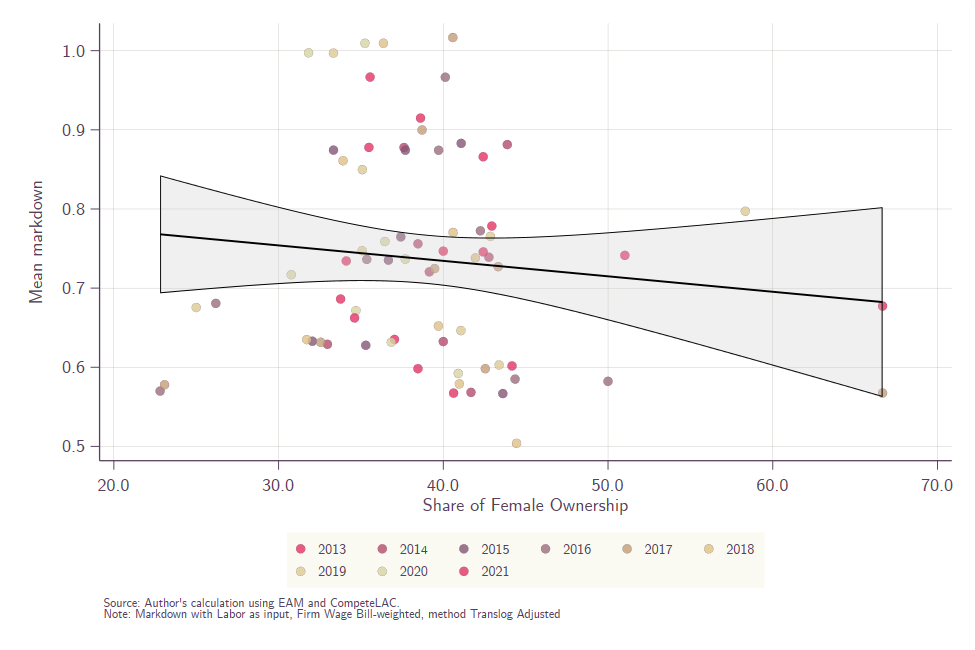
\includegraphics[width=\linewidth]{industry_markdown_femownshare.png}
\end{minipage}\hfill
\begin{minipage}{0.35\textwidth}
    \textbf{Preliminary findings:}
    Negative but not significant correlation between industry-level markdowns
    and female ownership share.
\end{minipage}
\end{figure}

\end{frame}


%%%%%%----------------------%%%%%%
\begin{frame}{Conclusion and Open Questions}
This paper examines how female ownership relates to labor markdowns. It highlights that firms often exert labor market power rather than behaving as pure wage takers.

\textbf{Open questions:}
\begin{itemize}
  \item Do results change when moving from industry-level to firm-level data?
  \item Is the negative relationship driven by higher productivity in female-led firms rather than wage setting alone?
  \begin{itemize}
    \item In Colombia female leadership is associated with higher firm performance (\cite{moreno-gomez_relationship_2018}). Larger, more productive firms pay higher wages, yet relative to workers' contributions to the value of the firm, the ratio might be larger, leading to higher markdowns.
  \end{itemize}
  \item Are effects stronger in more concentrated or friction-intensive labor markets? I would include industry HHI in the regression.
\end{itemize}
\end{frame}

\begin{frame}[allowframebreaks]{References}
\footnotesize
\bibliographystyle{apalike}
\bibliography{spring2026.bib}
\end{frame}
\end{document}